
\documentclass[11pt]{article}
\usepackage[T1]{fontenc}
\usepackage[utf8]{inputenc}
\usepackage{lmodern}
\usepackage{microtype}
\usepackage{amsmath,amssymb}
\usepackage{geometry}
\usepackage{tikz}
\usepackage{caption}
\usetikzlibrary{arrows.meta,calc}
\geometry{letterpaper,top=0.92in,bottom=0.98in,left=0.95in,right=0.95in}
\setlength{\parindent}{1.15em}
\setlength{\parskip}{0pt}
\emergencystretch=3em
\tolerance=1600
\hyphenpenalty=50
\exhyphenpenalty=50
\raggedbottom
\allowdisplaybreaks

\newcommand{\dd}{\,d}
\newcommand{\etal}{\eta}
\newcommand{\visviva}{\emph{vis viva}}

\captionsetup{font=small,labelformat=empty}
\hyphenation{ther-mo-dy-nam-ic dis-si-pa-ted iso-ther-mal iso-pi-es-tic con-den-sa-tion}
\begin{document}

\begin{center}
{\large II.}\par\vspace{1.1em}
{\Large\bfseries A METHOD OF GEOMETRICAL REPRESENTATION OF THE\\
THERMODYNAMIC PROPERTIES OF SUBSTANCES BY\\
MEANS OF SURFACES}\par\vspace{0.7em}
{\itshape Transactions of the Connecticut Academy, II. pp. 382--404, Dec. 1873.}
\end{center}

\setcounter{page}{33}

The leading thermodynamic properties of a fluid are determined by the relations which exist between the volume, pressure, temperature, energy, and entropy of a given mass of the fluid in a state of thermodynamic equilibrium. The same is true of a solid in regard to those properties which it exhibits in processes in which the pressure is the same in every direction about any point of the solid. But all the relations existing between these five quantities for any substance (three independent relations) may be deduced from the single relation existing for that substance between the volume, energy, and entropy. This may be done by means of the general equation,
\begin{equation}
\dd e=t\,\dd\eta-p\,\dd v, \tag{1}
\end{equation}
that is,
\begin{equation}
p=-\left(\frac{\dd e}{\dd v}\right)_\eta, \tag{2}
\end{equation}
\begin{equation}
t=\left(\frac{\dd e}{\dd\eta}\right)_v, \tag{3}
\end{equation}
where $v$, $p$, $t$, $e$, and $\eta$ denote severally the volume, pressure, absolute temperature, energy, and entropy of the body considered. The subscript letter after the differential coefficient indicates the quantity which is supposed constant in the differentiation.\footnote{For the demonstration of this equation, and in regard to the units used in the measurement of the quantities, the reader is referred to page 2.}

\begin{center}
\itshape Representation of Volume, Entropy, Energy, Pressure, and Temperature.
\end{center}

Now the relation between the volume, entropy, and energy may be represented by a surface, most simply if the rectangular co-ordinates of the various points of the surface are made equal to the volume, entropy, and energy of the body in its various states. It may be interesting to examine the properties of such a surface, which we will call the thermodynamic surface of the body for which it is formed.\footnote{Professor J. Thomson has proposed and used a surface in which the co-ordinates are proportional to the volume, pressure, and temperature of the body. (\emph{Proc. Roy. Soc.}, Nov. 16, 1871, vol. xx, p. 1; and \emph{Phil. Mag.}, vol. xliii, p. 227.) It is evident, however, that the relation between the volume, pressure, and temperature affords a less complete knowledge of the properties of the body than the relation between the volume, entropy, and energy. For, while the former relation is entirely determined by the latter, and can be derived from it by differentiation, the latter relation is by no means determined by the former.}

To fix our ideas, let the axes of $v$, $\eta$, and $e$ have the directions usually given to the axes of $X$, $Y$, and $Z$ ($v$ increasing to the right, $\eta$ forward, and $e$ upward). Then the pressure and temperature of the state represented by any point of the surface are equal to the tangents of the inclinations of the surface to the horizon at that point, as measured in planes perpendicular to the axes of $\eta$ and of $v$ respectively. (Eqs. 2 and 3.) It must be observed, however, that in the first case the angle of inclination is measured upward from the direction of decreasing $v$, and in the second, upward from the direction of increasing $\eta$. Hence, the tangent plane at any point indicates the temperature and pressure of the state represented. It will be convenient to speak of a plane as representing a certain pressure and temperature, when the tangents of its inclinations to the horizon, measured as above, are equal to that pressure and temperature.

Before proceeding farther, it may be worth while to distinguish between what is essential and what is arbitrary in a surface thus formed. The position of the plane $v=0$ in the surface is evidently fixed, but the position of the planes $\eta=0$, $e=0$ is arbitrary, provided the direction of the axes of $\eta$ and $e$ be not altered. This results from the nature of the definitions of entropy and energy, which involve each an arbitrary constant. As we may make $\eta=0$ and $e=0$ for any state of the body which we may choose, we may place the origin of co-ordinates at any point in the plane $v=0$. Again, it is evident from the form of equation (1) that whatever changes we may make in the units in which volume, entropy, and energy are measured, it will always be possible to make such changes in the units of temperature and pressure, that the equation will hold true in its present form, without the introduction of constants. It is easy to see how a change of the units of volume, entropy, and energy would affect the surface. The projections parallel to any one of the axes of distances between points of the surface would be changed in the ratio inverse to that in which the corresponding unit had been changed. These considerations enable us to foresee to a certain extent the nature of the general properties of the surface which we are to investigate. They must be such, namely, as shall not be affected by any of the changes mentioned above. For example, we may find properties which concern the plane $v=0$ (as that the whole surface must necessarily fall on the positive side of this plane), but we must not expect to find properties which concern the planes $\eta=0$, or $e=0$, in distinction from others parallel to them. It may be added that, as the volume, entropy, and energy of a body are equal to the sums of the volumes, entropies, and energies of its parts, if the surface should be constructed for bodies differing in quantity but not in kind of matter, the different surfaces thus formed would be similar to one another, their linear dimensions being proportional to the quantities of matter.

\begin{center}
\itshape Nature of that Part of the Surface which represents States which are not Homogeneous.
\end{center}

This mode of representation of the volume, entropy, energy, pressure, and temperature of a body will apply as well to the case in which different portions of the body are in different states (supposing always that the whole is in a state of thermodynamic equilibrium), as to that in which the body is uniform in state throughout. For the body taken as a whole has a definite volume, entropy, and energy, as well as pressure and temperature, and the validity of the general equation (1) is independent of the uniformity or diversity in respect to state of the different portions of the body.\footnote{It is, however, supposed in this equation that the variations in the state of the body, to which $\dd v$, $\dd\eta$, and $\dd e$ refer, are such as may be produced reversibly by expansion and compression or by addition and subtraction of heat. Hence, when the body consists of parts in different states, it is necessary that these states should be such as can pass either into the other without sensible change of pressure or temperature. Otherwise, it would be necessary to suppose in the differential equation (1) that the proportion in which the body is divided into the different states remains constant. But such a limitation would render the equation as applied to a compound of different states valueless for our present purpose. If, however, we leave out of account the cases in which we regard the states as chemically different from one another, which lie beyond the scope of this paper, experience justifies us in assuming the above condition (that either of the two states existing in contact can pass into the other without sensible change of the pressure or temperature), as at least approximately true, when one of the states is fluid. But if both are solid, the necessary mobility of the parts is wanting. It must therefore be understood, that the following discussion of the compound states is not intended to apply without limitation to the exceptional cases, where we have two different solid states of the same substance at the same pressure and temperature. It may be added that the thermodynamic equilibrium which subsists between two such solid states of the same substance differs from that which subsists when one of the states is fluid, very much as in statics an equilibrium which is maintained by friction differs from that of a frictionless machine in which the active forces are so balanced, that the slightest change of force will produce motion in either direction. Another limitation is rendered necessary by the fact that in the following discussion the magnitude and form of the bounding and dividing surfaces are left out of account; so that the results are in general strictly valid only in cases in which the influence of these particulars may be neglected. When, therefore, two states of the substance are spoken of as in contact, it must be understood that the surface dividing them is plane. To consider the subject in a more general form, it would be necessary to introduce considerations which belong to the theories of capillarity and crystallization.} It is evident, therefore, that the thermodynamic surface, for many substances at least, can be divided into two parts, of which one represents the homogeneous states, the other those which are not so. We shall see that, when the former part of the surface is given, the latter can readily be formed, as indeed we might expect. We may therefore call the former part the primitive surface, and the latter the derived surface.

To ascertain the nature of the derived surface and its relations to the primitive surface sufficiently to construct it when the latter is given, it is only necessary to use the principle that the volume, entropy, and energy of the whole body are equal to the sums of the volumes, entropies, and energies respectively of the parts, while the pressure and temperature of the whole are the same as those of each of the parts. Let us commence with the case in which the body is in part solid, in part liquid, and in part vapor. The position of the point determined by the volume, entropy, and energy of such a compound will be that of the center of gravity of masses proportioned to the masses of solid, liquid, and vapor placed at the three points of the primitive surface which represent respectively the states of complete solidity, complete liquidity, and complete vaporization, each at the temperature and pressure of the compound. Hence, the part of the surface which represents a compound of solid, liquid, and vapor is a plane triangle, having its vertices at the points mentioned. The fact that the surface is here plane indicates that the pressure and temperature are here constant, the inclination of the plane indicating the value of these quantities. Moreover, as these values are the same for the compound as for the three different homogeneous states corresponding to its different portions, the plane of the triangle is tangent at each of its vertices to the primitive surface, viz.: at one vertex to that part of the primitive surface which represents solid, at another to the part representing liquid, and at the third to the part representing vapor.

When the body consists of a compound of two different homogeneous states, the point which represents the compound state will be at the center of gravity of masses proportioned to the masses of the parts of the body in the two different states and placed at the points of the primitive surface which represent these two states (i.e., which represent the volume, entropy, and energy of the body, if its whole mass were supposed successively in the two homogeneous states which occur in its parts). It will therefore be found upon the straight line which unites these two points. As the pressure and temperature are evidently constant for this line, a single plane can be tangent to the derived surface throughout this line and at each end of the line tangent to the primitive surface.\footnote{It is here shown that, if two different states of the substance are such that they can exist permanently in contact with each other, the points representing these states in the thermodynamic surface have a common tangent plane. We shall see hereafter that the converse of this is true,--that, if two points in the thermodynamic surface have a common tangent plane, the states represented are such as can permanently exist in contact; and we shall also see what determines the direction of the discontinuous change which occurs when two different states of the same pressure and temperature, for which the condition of a common tangent plane is not satisfied, are brought into contact.

It is easy to express this condition analytically. Resolving it into the conditions, that the tangent planes shall be parallel, and that they shall cut the axis of $e$ at the same point, we have the equations
\begin{align}
p'&=p'', \tag{\ensuremath{\alpha}}\\
t'&=t'', \tag{\ensuremath{\beta}}\\
e'-t'\eta'+p'v'&=e''-t''\eta''+p''v'', \tag{\ensuremath{\gamma}}
\end{align}
where the letters which refer to the different states are distinguished by accents. If there are three states which can exist in contact, we must have for these states,
\begin{align*}
p'&=p''=p''',\\
t'&=t''=t''',\\
e'-t'\eta'+p'v'&=e''-t''\eta''+p''v''=e'''-t'''\eta'''+p'''v'''.
\end{align*}
These results are interesting, as they show us how we might foresee whether two given states of a substance of the same pressure and temperature can or cannot exist in contact. It is indeed true, that the values of $e$ and $\eta$ cannot like those of $v$, $p$, and $t$ be ascertained by mere measurements upon the substance while in the two states in question. It is necessary, in order to find the value of $e''-e'$ or $\eta''-\eta'$, to carry out measurements upon a process by which the substance is brought from one state to the other, but this need not be by a process in which the two given states shall be found in contact, and in some cases at least it may be done by processes in which the body remains always homogeneous in state. For we know by the experiments of Dr. Andrews, \emph{Phil. Trans.}, vol. 159, p. 575, that carbonic acid may be carried from any of the states which we usually call liquid to any of those which we usually call gas, without losing its homogeneity. Now, if we had so carried it from a state of liquidity to a state of gas of the same pressure and temperature, making the proper measurements in the process, we should be able to foretell what would occur if these two states of the substance should be brought together,--whether evaporation would take place, or condensation, or whether they would remain unchanged in contact,--although we had never seen the phenomenon of the coexistence of these two states, or of any other two states of this substance.

Equation ($\gamma$) may be put in a form in which its validity is at once manifest for two states which can pass either into the other at a constant pressure and temperature. If we put $p'$ and $t'$ for the equivalent $p''$ and $t''$, the equation may be written
\[
e''-e'=t'(\eta''-\eta')-p'(v''-v').
\]
Here the left hand member of the equation represents the difference of energy in the two states, and the two terms on the right represent severally the heat received and the work done when the body passes from one state to the other. The equation may also be derived at once from the general equation (1) by integration.

It is well known that when the two states being both fluid meet in a curved surface, instead of ($\alpha$) we have
\[
p''-p'=T\left(\frac{1}{r}+\frac{1}{r'}\right),
\]
where $r$ and $r'$ are the radii of the principal curvatures of the surface of contact at any point (positive, if the concavity is toward the mass to which $p''$ refers), and $T$ is what is called the superficial tension. Equation ($\beta$), however, holds good for such cases, and it might easily be proved that the same is true of equation ($\gamma$). In other words, the tangent planes for the points in the thermodynamic surface representing the two states cut the plane $v=0$ in the same line.} If we now imagine the temperature and pressure of the compound to vary, the two points of the primitive surface, the line in the derived surface uniting them, and the tangent plane will change their positions, maintaining the aforesaid relations. We may conceive of the motion of the tangent plane as produced by rolling upon the primitive surface, while tangent to it in two points, and as it is also tangent to the derived surface in the lines joining these points, it is evident that the latter is a developable surface and forms a part of the envelop of the successive positions of the rolling plane. We shall see hereafter that the form of the primitive surface is such that the double tangent plane does not cut it, so that this rolling is physically possible.

From these relations may be deduced by simple geometrical considerations one of the principal propositions in regard to such compounds. Let the tangent plane touch the primitive surface at the two points $L$ and $V$ (fig. 1), which, to fix our ideas, we may suppose to represent liquid and vapor; let planes pass through these points perpendicular to the axes of $v$ and $\eta$ respectively, intersecting in the line $AB$, which will be parallel to the axis of $e$. Let the tangent plane cut this line at $A$, and let $LB$ and $VC$ be drawn at right angles to $AB$ and parallel to the axes of $\eta$ and $v$. Now the pressure and temperature represented by the tangent plane are evidently $AC/CV$ and $AB/BL$ respectively, and if we suppose the tangent plane in rolling upon the primitive surface to turn about its instantaneous axis $LV$ an infinitely small angle, so as to meet $AB$ in $A'$, $dp$ and $dt$ will be equal to $AA'/CV$ and $AA'/BL$ respectively. Therefore,

\begin{figure}[h]
\centering
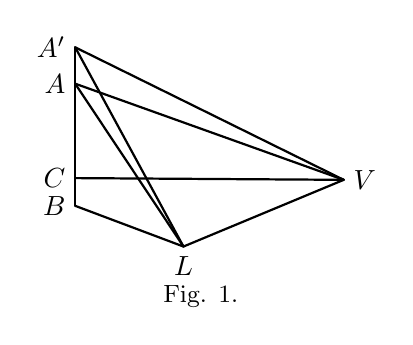
\begin{tikzpicture}[scale=1.1,line cap=round,line join=round]
\coordinate (Ap) at (0,2.25);
\coordinate (A) at (0,1.83);
\coordinate (C) at (0,0.74);
\coordinate (B) at (0,0.42);
\coordinate (L) at (1.25,-0.05);
\coordinate (V) at (3.10,0.72);
\draw[thick] (B)--(Ap);
\draw[thick] (Ap)--(V)--(L)--(B);
\draw[thick] (A)--(V);
\draw[thick] (A)--(L);
\draw[thick] (C)--(V);
\draw[thick] (Ap)--(L);
\node[left] at (Ap) {$A'$};
\node[left] at (A) {$A$};
\node[left] at (C) {$C$};
\node[left] at (B) {$B$};
\node[below] at (L) {$L$};
\node[right] at (V) {$V$};
\node at (1.45,-0.63) {\small Fig. 1.};
\end{tikzpicture}
\end{figure}

\[
\frac{dp}{dt}=\frac{BL}{CV}=\frac{\eta''-\eta'}{v''-v'},
\]
where $v'$ and $\eta'$ denote the volume and entropy for the point $L$, and $v''$ and $\eta''$ those for the point $V$. If we substitute for $\eta''-\eta'$ its equivalent $r/t$ ($r$ denoting the heat of vaporization), we have the equation in its usual form,
\[
\frac{dp}{dt}=\frac{r}{t(v''-v')}.
\]

\begin{center}
\itshape Properties of the Surface relating to Stability of Thermodynamic Equilibrium.
\end{center}

We will now turn our attention to the geometrical properties of the surface, which indicate whether the thermodynamic equilibrium of the body is stable, unstable, or neutral. This will involve the consideration, to a certain extent, of the nature of the processes which take place when equilibrium does not subsist. We will suppose the body placed in a medium of constant pressure and temperature; but as, when the pressure or temperature of the body at its surface differs from that of the medium, the immediate contact of the two is hardly consistent with the continuance of the initial pressure and temperature of the medium, both of which we desire to suppose constant, we will suppose the body separated from the medium by an envelop which will yield to the smallest differences of pressure between the two, but which can only yield very gradually, and which is also a very poor conductor of heat. It will be convenient and allowable for the purposes of reasoning to limit its properties to those mentioned, and to suppose that it does not occupy any space, or absorb any heat except what it transmits, i.e., to make its volume and its specific heat $0$. By the intervention of such an envelop, we may suppose the action of the body upon the medium to be so retarded as not sensibly to disturb the uniformity of pressure and temperature in the latter.

When the body is not in a state of thermodynamic equilibrium, its state is not one of those which are represented by our surface. The body, however, as a whole has a certain volume, entropy, and energy, which are equal to the sums of the volumes, etc., of its parts.\footnote{As the discussion is to apply to cases in which the parts of the body are in (sensible) motion, it is necessary to define the sense in which the word energy is to be used. We will use the word as including the \visviva{} of sensible motions.} If, then, we suppose points endowed with mass proportional to the masses of the various parts of the body, which are in different thermodynamic states, placed in the positions determined by the states and motions of these parts, (i.e., so placed that their co-ordinates are equal to the volume, entropy, and energy of the whole body supposed successively in the same states and endowed with the same velocities as the different parts), the center of gravity of such points thus placed will evidently represent by its co-ordinates the volume, entropy, and energy of the whole body. If all parts of the body are at rest, the point representing its volume, entropy, and energy will be the center of gravity of a number of points upon the primitive surface. The effect of motion in the parts of the body will be to move the corresponding points parallel to the axis of $e$, a distance equal in each case to the \visviva{} of the whole body, if endowed with the velocity of the part represented;--the center of gravity of points thus determined will give the volume, entropy, and energy of the whole body.

Now let us suppose that the body having the initial volume, entropy, and energy, $v'$, $\eta'$, and $e'$, is placed (enclosed in an envelop as aforesaid) in a medium having the constant pressure $P$ and temperature $T$, and by the action of the medium and the interaction of its own parts comes to a final state of rest in which its volume, etc., are $v''$, $\eta''$, $e''$;--we wish to find a relation between these quantities. If we regard, as we may, the medium as a very large body, so that imparting heat to it or compressing it within moderate limits will have no appreciable effect upon its pressure and temperature, and write $V$, $H$, and $E$, for its volume, entropy, and energy, equation (1) becomes
\[
\dd E=T\,\dd H-P\,\dd V,
\]
which we may integrate regarding $P$ and $T$ as constants, obtaining
\begin{equation}
E''-E'=TH''-TH'-PV''+PV', \tag{a}
\end{equation}
where $E'$, $E''$, etc., refer to the initial and final states of the medium. Again, as the sum of the energies of the body and the surrounding medium may become less, but cannot become greater (this arises from the nature of the envelop supposed), we have
\begin{equation}
e''+E''\le e'+E'. \tag{b}
\end{equation}
Again as the sum of the entropies may increase but cannot diminish,
\begin{equation}
\eta''+H''\ge \eta'+H'. \tag{c}
\end{equation}
Lastly, it is evident that
\begin{equation}
v''+V''=v'+V'. \tag{d}
\end{equation}
These four equations may be arranged with slight changes as follows:
\begin{align*}
-E''+TH''-PV''&=-E'+TH'-PV',\\
e''+E''&\le e'+E',\\
-T\eta''-TH''&\le -T\eta'-TH',\\
Pv''+PV''&=Pv'+PV'.
\end{align*}
By addition we have
\begin{equation}
e''-T\eta''+Pv''\le e'-T\eta'+Pv'. \tag{e}
\end{equation}
Now the two members of this equation evidently denote the vertical distances of the points $(v'',\eta'',e'')$ and $(v',\eta',e')$ above the plane passing through the origin and representing the pressure $P$ and temperature $T$. And the equation expresses that the ultimate distance is less or at most equal to the initial. It is evidently immaterial whether the distances be measured vertically or normally, or that the fixed plane representing $P$ and $T$ should pass through the origin; but distances must be considered negative when measured from a point below the plane.

It is evident that the sign of inequality holds in (e) if it holds in either (b) or (c), therefore, it holds in (e) if there are any differences of pressure or temperature between the different parts of the body or between the body and the medium, or if any part of the body has sensible motion. (In the latter case, there would be an increase of entropy due to the conversion of this motion into heat.) But even if the body is initially without sensible motion and has throughout the same pressure and temperature as the medium, the sign $<$ will still hold if different parts of the body are in states represented by points in the thermodynamic surface at different distances from the fixed plane representing $P$ and $T$. For it certainly holds if such initial circumstances are followed by differences of pressure or temperature, or by sensible velocities. Again, the sign of inequality would necessarily hold if one part of the body should pass, without producing changes of pressure or temperature or sensible velocities, into the state of another part represented by a point not at the same distance from the fixed plane representing $P$ and $T$. But these are the only suppositions possible in the case, unless we suppose that equilibrium subsists, which would require that the points in question should have a common tangent plane (page 37), whereas by supposition the planes tangent at the different points are parallel but not identical.

The results of the preceding paragraph may be summed up as follows:--Unless the body is initially without sensible motion, and its state, if homogeneous, is such as is represented by a point in the primitive surface where the tangent plane is parallel to the fixed plane representing $P$ and $T$, or, if the body is not homogeneous in state, unless the points in the primitive surface representing the states of its parts have a common tangent plane parallel to the fixed plane representing $P$ and $T$, such changes will ensue that the distance of the point representing the volume, entropy, and energy of the body from that fixed plane will be diminished (distances being considered negative if measured from points beneath the plane). Let us apply this result to the question of the stability of the body when surrounded, as supposed, by a medium of constant temperature and pressure.

The state of the body in equilibrium will be represented by a point in the thermodynamic surface, and as the pressure and temperature of the body are the same as those of the surrounding medium, we may take the tangent plane at that point as the fixed plane representing $P$ and $T$. If the body is not homogeneous in state, although in equilibrium, we may, for the purposes of this discussion of stability, either take a point in the derived surface as representing its state, or we may take the points in the primitive surface which represent the states of the different parts of the body. These points, as we have seen (page 37), have a common tangent plane, which is identical with the tangent plane for the point in the derived surface.

Now, if the form of the surface be such that it falls above the tangent plane except at the single point of contact, the equilibrium is necessarily stable; for if the condition of the body be slightly altered, either by imparting sensible motion to any part of the body, or by slightly changing the state of any part, or by bringing any small part into any other thermodynamic state whatever, or in all of these ways, the point representing the volume, entropy, and energy of the whole body will then occupy a position above the original tangent plane, and the proposition above enunciated shows that processes will ensue which will diminish the distance of this point from that plane, and that such processes cannot cease until the body is brought back into its original condition, when they will necessarily cease on account of the form supposed of the surface.

On the other hand, if the surface have such a form that any part of it falls below the fixed tangent plane, the equilibrium will be unstable. For it will evidently be possible by a slight change in the original condition of the body (that of equilibrium with the surrounding medium and represented by the point or points of contact) to bring the point representing the volume, entropy, and energy of the body into a position below the fixed tangent plane, in which case we see by the above proposition that processes will occur which will carry the point still farther from the plane, and that such processes cannot cease until all the body has passed into some state entirely different from its original state.

It remains to consider the case in which the surface, although it does not anywhere fall below the fixed tangent plane, nevertheless meets the plane in more than one point. The equilibrium in this case, as we might anticipate from its intermediate character between the cases already considered, is neutral. For if any part of the body be changed from its original state into that represented by another point in the thermodynamic surface lying in the same tangent plane, equilibrium will still subsist. For the supposition in regard to the form of the surface implies that uniformity in temperature and pressure still subsists, nor can the body have any necessary tendency to pass entirely into the second state or to return into the original state, for a change of the values of $T$ and $P$ less than any assignable quantity would evidently be sufficient to reverse such a tendency if any such existed, as either point at will could by such an infinitesimal variation of $T$ and $P$ be made the nearer to the plane representing $T$ and $P$.

It must be observed that in the case where the thermodynamic surface at a certain point is concave upward in both its principal
curvatures, but somewhere falls below the tangent plane drawn through that point, the equilibrium although unstable in regard to discontinuous changes of state is stable in regard to continuous changes, as appears on restricting the test of stability to the vicinity of the point in question; that is, if we suppose a body to be in a state represented by such a point, although the equilibrium would show itself unstable if we should introduce into the body a small portion of the same substance in one of the states represented by points below the tangent plane, yet if the conditions necessary for such a discontinuous change are not present, the equilibrium would be stable. A familiar example of this is afforded by liquid water when heated at any pressure above the temperature of boiling water at that pressure.\footnote{If we wish to express in a single equation the necessary and sufficient condition of thermodynamic equilibrium for a substance when surrounded by a medium of constant pressure $P$ and temperature $T$, this equation may be written
\[
\delta(e-T\eta+Pv)=0,
\]
when $\delta$ refers to the variation produced by any variations in the state of the parts of the body, and (when different parts of the body are in different states) in the proportion in which the body is divided between the different states. The condition of stable equilibrium is that the value of the expression in the parenthesis shall be a minimum.}

\begin{center}
\itshape Leading Features of the Thermodynamic Surface for Substances which take the forms of Solid, Liquid, and Vapor.
\end{center}

We are now prepared to form an idea of the general character of the primitive and derived surfaces and their mutual relations for a substance which takes the forms of solid, liquid, and vapor. The primitive surface will have a triple tangent plane touching it at the three points which represent the three states which can exist in contact. Except at these three points, the primitive surface falls entirely above the tangent plane. That part of the plane which forms a triangle having its vertices at the three points of contact, is the derived surface which represents a compound of the three states of the substance. We may now suppose the plane to roll on the under side of the surface, continuing to touch it in two points without cutting it. This it may do in three ways, viz: it may commence by turning about any one of the sides of the triangle aforesaid. Any pair of points which the plane touches at once represent states which can exist permanently in contact. In this way six lines are traced upon the surface. These lines have in general a common property, that a tangent plane at any point in them will also touch the surface in another point. We must say \emph{in general}, for, as we shall see hereafter, this statement does not hold good for the critical point. A tangent plane at any point of the surface outside of these lines has the surface entirely above it, except the single point of contact. A tangent plane at any point of the primitive surface within these lines will cut the surface. These lines, therefore, taken together may be called the \emph{limit of absolute stability}, and the surface outside of them, the \emph{surface of absolute stability}. That part of the envelop of the rolling plane, which lies between the pair of lines which the plane traces on the surface, is a part of the derived surface, and represents a mixture of two states of the substance.

The relations of these lines and surfaces are roughly represented in horizontal projection\footnote{A horizontal projection of the thermodynamic surface is identical with the diagram described on pages 20--28 of this volume, under the name of the volume-entropy diagram.} in figure 2, in which the full lines represent lines on the primitive surface, and the dotted lines those on the derived surface. $S$, $L$, and $V$ are the points which have a common tangent plane and represent the states of solid, liquid, and vapor which can exist in contact.

\begin{figure}[htbp]
\centering
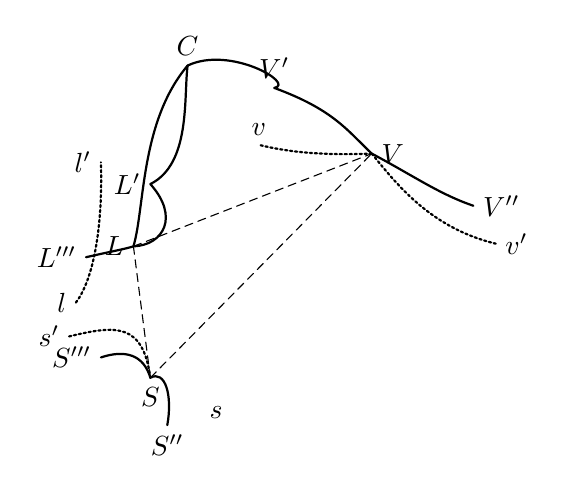
\begin{tikzpicture}[scale=.86, line cap=round, line join=round, >=Stealth]
  \coordinate (C) at (0,3.45);
  \coordinate (L) at (-.80,.78);
  \coordinate (Lp) at (-.55,1.70);
  \coordinate (Lppp) at (-1.50,.62);
  \coordinate (ldot) at (-1.65,-.05);
  \coordinate (ldotp) at (-1.28,2.02);
  \coordinate (V) at (2.72,2.15);
  \coordinate (Vp) at (1.28,3.12);
  \coordinate (Vpp) at (4.22,1.38);
  \coordinate (vdot) at (4.55,.82);
  \coordinate (vdotp) at (1.05,2.28);
  \coordinate (S) at (-.55,-1.16);
  \coordinate (Spp) at (-.30,-1.86);
  \coordinate (Sppp) at (-1.28,-.86);
  \coordinate (sdot) at (.18,-1.68);
  \coordinate (sdotp) at (-1.75,-.55);
  \draw[thick] (Lppp).. controls (-1.15,.70) and (-.93,.74)..(L).. controls (-.63,1.35) and (-.70,2.62)..(C);
  \draw[thick] (C).. controls (.63,3.75) and (1.60,3.18)..(Vp).. controls (2.15,2.80) and (2.35,2.50)..(V).. controls (3.34,1.82) and (3.72,1.55)..(Vpp);
  \draw[thick] (L).. controls (-.35,.80) and (-.12,1.22)..(Lp).. controls (.05,2.00) and (-.06,2.98)..(C);
  \draw[thick] (Sppp).. controls (-.92,-.74) and (-.65,-.82)..(S).. controls (-.33,-1.04) and (-.22,-1.42)..(Spp);
  \draw[densely dotted, thick] (ldot).. controls (-1.42,.25) and (-1.25,.95)..(ldotp);
  \draw[densely dotted, thick] (sdotp).. controls (-1.05,-.38) and (-.66,-.35)..(S);
  \draw[densely dotted, thick] (V).. controls (3.10,1.68) and (3.60,1.05)..(vdot);
  \draw[densely dotted, thick] (V).. controls (1.92,2.12) and (1.46,2.18)..(vdotp);
  \draw[densely dashed] (L)--(V);
  \draw[densely dashed] (S)--(V);
  \draw[densely dashed] (S)--(L);
  \node[above] at (C) {$C$};
  \node[left] at (L) {$L$};
  \node[left] at (Lp) {$L'$};
  \node[left] at (Lppp) {$L'''$};
  \node[left] at (ldot) {$l$};
  \node[left] at (ldotp) {$l'$};
  \node[right] at (V) {$V$};
  \node[above] at (Vp) {$V'$};
  \node[right] at (Vpp) {$V''$};
  \node[right] at (vdot) {$v'$};
  \node[above] at (vdotp) {$v$};
  \node[below] at (S) {$S$};
  \node[left] at (Sppp) {$S'''$};
  \node[below] at (Spp) {$S''$};
  \node[right] at (sdot) {$s$};
  \node[left] at (sdotp) {$s'$};
\end{tikzpicture}
\caption{Fig. 2.}
\end{figure}

The plane triangle $SLV$ is the derived surface representing compounds of these states. $LL'$ and $VV'$ are the pair of lines traced by the rolling double tangent plane, between which lies the derived surface representing compounds of liquid and vapor. $VV''$ and $SS''$ are another such pair, between which lies the derived surface representing compounds of vapor and solid. $SS'''$ and $LL'''$ are the third pair, between which lies the derived surface representing a compound of solid and liquid. $L'''LL'$, $V'VV''$ and $S''SS'''$ are the boundaries of the surfaces which represent respectively the absolutely stable states of liquid, vapor, and solid.

The geometrical expression of the results which Dr. Andrews, \emph{Phil. Trans.}, vol. 159, p. 575, has obtained by his experiments with carbonic acid is that, in the case of this substance at least, the derived surface which represents a compound of liquid and vapor is terminated as follows: as the tangent plane rolls upon the primitive surface, the two points of contact approach one another and finally fall together. The rolling of the double tangent plane necessarily comes to an end. The point where the two points of contact fall together is the \emph{critical point}. Before considering farther the geometrical characteristics of this point and their physical significance, it will be convenient to investigate the nature of the primitive surface which lies between the lines which form the limit of absolute stability.

Between two points of the primitive surface which have a common tangent plane, as those represented by $L'$ and $V'$ in figure 2, if there is no gap in the primitive surface, there must evidently be a region where the surface is concave toward the tangent plane in one of its principal curvatures at least, and therefore represents states of unstable equilibrium in respect to continuous as well as discontinuous changes (see pages 42, 43).\footnote{This is the same result as that obtained by Professor J. Thomson in connection with the surface referred to in the note on page 34.} If we draw a line upon the primitive surface, dividing it into parts which represent respectively stable and unstable equilibrium, in respect to continuous changes, i.e., dividing the surface which is concave upward in both its principal curvatures from that which is concave downward in one or both, this line, which may be called the \emph{limit of essential instability}, must have a form somewhat like that represented by $ll'Cvv'ss'$ in figure 2. It touches the limit of absolute stability at the critical point $C$. For we may take a pair of points in $LC$ and $VC$ having a common tangent plane as near to $C$ as we choose, and the line joining them upon the primitive surface made by a plane section perpendicular to the tangent plane, will pass through an area of instability.

The geometrical properties of the critical point in our surface may be made more clear by supposing the lines of curvature drawn upon the surface for one of the principal curvatures, that one, namely, which has different signs upon different sides of the limit of essential instability. The lines of curvature which meet this line will in general cross it. At any point where they do so, as the sign of their curvature changes, they evidently cut a plane tangent to the surface, and therefore the surface itself cuts the tangent plane. But where one of these lines of curvature touches the limit of essential instability without crossing it, so that its curvature remains always positive (curvatures being considered positive when the concavity is on the upper side of the surface), the surface evidently does not cut the tangent plane, but has a contact of the third order with it in the section of least curvature. The critical point, therefore, must be a point where the line of that principal curvature which changes its sign is tangent to the line which separates positive from negative curvatures.

From the last paragraphs we may derive the following physical property of the critical state:---Although this is a limiting state between those of stability and those of instability in respect to continuous changes, and although such limiting states are in general unstable in respect to such changes, yet the critical state is stable in regard to them. A similar proposition is true in regard to absolute stability, i.e., if we disregard the distinction between continuous and discontinuous changes, viz: that although the critical state is a limiting state between those of stability and instability, and although the equilibrium of such limiting states is in general neutral (when we suppose the substance surrounded by a medium of constant pressure and temperature), yet the critical point is stable.

From what has been said of the curvature of the primitive surface at the critical point, it is evident, that if we take a point in this surface infinitely near to the critical point, and such that the tangent planes for these two points shall intersect in a line perpendicular to the section of least curvature at the critical point, the angle made by the two tangent planes will be an infinitesimal of the same order as the cube of the distance of these points. Hence, at the critical point
\begin{align*}
\left(\frac{dp}{dv}\right)_t&=0,&
\left(\frac{dp}{d\eta}\right)_t&=0,&
\left(\frac{dt}{dv}\right)_p&=0,&
\left(\frac{dt}{d\eta}\right)_p&=0,\\[0.35em]
\left(\frac{d^2p}{dv^2}\right)_t&=0,&
\left(\frac{d^2p}{d\eta^2}\right)_t&=0,&
\left(\frac{d^2t}{dv^2}\right)_p&=0,&
\left(\frac{d^2t}{d\eta^2}\right)_p&=0,
\end{align*}
and if we imagine the isothermal and isopiestic (line of constant pressure) drawn for the critical point upon the primitive surface, these lines will have a contact of the second order.

Now the elasticity of the substance at constant temperature and its specific heat at constant pressure may be defined by the equations,
\[
\varepsilon=-v\left(\frac{dp}{dv}\right)_t,
\qquad
s=t\left(\frac{d\eta}{dt}\right)_p;
\]
therefore at the critical point
\[
\varepsilon=0,
\qquad
\frac{1}{s}=0,
\]
\[
\left(\frac{d\varepsilon}{dv}\right)_t=0,
\qquad
\left(\frac{d\varepsilon}{d\eta}\right)_t=0,
\qquad
\left(\frac{d(s^{-1})}{dv}\right)_p=0,
\qquad
\left(\frac{d(s^{-1})}{d\eta}\right)_p=0.
\]
The last four equations would also hold good if $p$ were substituted for $t$, and \emph{vice versa}.

We have seen that in the case of such substances as can pass continuously from the state of liquid to that of vapor, unless the primitive surface is abruptly terminated, and that in a line which passes through the critical point, a part of it must represent states which are essentially unstable (i.e., unstable in regard to continuous changes), and therefore cannot exist permanently unless in very limited spaces. It does not necessarily follow that such states cannot be realized at all. It appears quite probable, that a substance initially in the critical state may be allowed to expand so rapidly that, the time being too short for appreciable conduction of heat, it will pass into some of these states of essential instability. No other result is possible on the supposition of no transmission of heat, which requires that the points representing the states of all the parts of the body shall be confined to the isentropic (adiabatic) line of the critical point upon the primitive surface. It will be observed that there is no instability in regard to changes of state thus limited, for this line (the plane section of the primitive surface perpendicular to the axis of $\eta$) is concave upward, as is evident from the fact that the primitive surface lies entirely above the tangent plane for the critical point.

We may suppose waves of compression and expansion to be propagated in a substance initially in the critical state. The velocity of propagation will depend upon the value of $\left(dp/dv\right)_\eta$, i.e., of $-\left(d^2e/dv^2\right)_\eta$. Now for a wave of compression the value of these expressions is determined by the form of the isentropic on the primitive surface. If a wave of expansion has the same velocity approximately as one of compression, it follows that the substance when expanded under the circumstances remains in a state represented by the primitive surface, which involves the realization of states of essential instability. The value of $\left(d^2e/dv^2\right)_\eta$ in the derived surface is, it will be observed, totally different from its value in the primitive surface, as the curvature of these surfaces at the critical point is different.

The case is different in regard to the part of the surface between the limit of absolute stability and the limit of essential instability. Here, we have experimental knowledge of some of the states represented. In water, for example, it is well known that liquid states can be realized beyond the limit of absolute stability,---both beyond the part of the limit where vaporization usually commences ($LL'$ in figure 2), and beyond the part where congelation usually commences ($LL'''$). That vapor may also exist beyond the limit of absolute stability, i.e., that it may exist at a given temperature at pressures greater than that of equilibrium between the vapor and its liquid meeting in a plane surface at that temperature, the considerations adduced by Sir W. Thomson in his paper ``On the equilibrium of a vapor at the curved surface of a liquid'' (\emph{Proc. Roy. Soc. Edinb.}, Session 1869--1870, and \emph{Phil. Mag.}, vol. xlii, p. 448), leave no room for doubt. By experiments like that suggested by Professor J. Thomson in his paper already referred to, we may be able to carry vapors farther beyond the limit of absolute stability.\footnote{If we experiment with a fluid which does not wet the vessel which contains it, we may avoid the necessity of keeping the vessel hotter than the vapor, in order to prevent condensation. If a glass bulb with a stem of sufficient length be placed vertically with the open end of the stem in a cup of mercury, the stem containing nothing but mercury and its vapor, and the bulb nothing but the vapor, the height at which the mercury rests in the stem, affords a ready and accurate means of determining the pressure of the vapor. If the stem at the top of the column of liquid should be made hotter than the bulb, condensation would take place in the latter, if the liquid were one which would wet the bulb. But as this is not the case, it appears probable, that if the experiment were conducted with proper precautions, there would be no condensation within certain limits in regard to the temperatures. If condensation should take place, it would be easily observed, especially if the bulb were bent over, so that the mercury condensed could not run back into the stem. So long as condensation does not occur, it will be easy to give any desired (different) temperatures to the bulb and the top of the column of mercury in the stem. The temperature of the latter will determine the pressure of the vapor in the bulb. In this way, it would appear, we may obtain in the bulb vapor of mercury having pressures greater for the temperatures than those of saturated vapor.} As the resistance to deformation characteristic of solids evidently tends to prevent a discontinuous change of state from commencing within them, substances can doubtless exist in solid states very far beyond the limit of absolute stability.

The surface of absolute stability, together with the triangle representing a compound of three states, and the three developable surfaces which have been described representing compounds of two states, forms a continuous sheet, which is everywhere concave upward except where it is plane, and has only one value of $e$ for any given values of $v$ and $\eta$. Hence, as $t$ is necessarily positive, it has only one value of $\eta$ for any given values of $v$ and $e$. If vaporization can take place at every temperature except $0$, $p$ is everywhere positive, and the surface has only one value of $v$ for any given values of $\eta$ and $e$. It forms the \emph{surface of dissipated energy}. If we consider all the points representing the volume, entropy, and energy of the body in every possible state, whether of equilibrium or not, these points will form a solid figure unbounded in some directions, but bounded in others by this surface.\footnote{This description of the surface of dissipated energy is intended to apply to a substance capable of existing as solid, liquid, and vapor, and which presents no anomalies in its thermodynamic properties. But, whatever the form of the primitive surface may be, if we take the parts of it for every point of which the tangent plane does not cut the primitive surface, together with all the plane and developable derived surfaces which can be formed in a manner analogous to those described in the preceding pages, by fixed and rolling tangent planes which do not cut the primitive surface,---such surfaces taken together will form a continuous sheet, which, if we reject the part, if any, for which $p<0$, forms the surface of dissipated energy and has the geometrical properties mentioned above.

There will, however, be no such part in which $p<0$, if there is any assignable temperature $t'$ at which the substance has the properties of a perfect gas except when its volume is less than a certain quantity $v'$. For the equations of an isothermal line in the thermodynamic surface of a perfect gas are (see equations (B) and (E) on pages 12--13)
\[
e=c,
\qquad
\eta=a\log v+C'.
\]
The isothermal of $t'$ in the thermodynamic surface of the substance in question must therefore have the same equations in the part in which $v$ exceeds the constant $v'$. Now if at any point in this surface $p<0$ and $t>0$ the equation of the tangent plane for that point will be
\[
e=m\eta+nv+C'',
\]
where $m$ denotes the temperature and $-n$ the pressure for the point of contact, so that $m$ and $n$ are both positive. Now it is evidently possible to give so large a value to $v$ in the equations of the isothermal that the point thus determined shall fall below the tangent plane. Therefore, the tangent plane cuts the primitive surface, and the point of the thermodynamic surface for which $p<0$ cannot belong to the surfaces mentioned in the last paragraph as forming a continuous sheet.}

The lines traced upon the primitive surface by the rolling double tangent plane, which have been called the limit of absolute stability, do not end at the vertices of the triangle which represents a mixture of those states. For when the plane is tangent to the primitive surface in these three points, it can commence to roll upon the surface as a double tangent plane not only by leaving the surface at one of these points, but also by a rotation in the opposite direction. In the latter case, however, the lines traced upon the primitive surface by the points of contact, although a continuation of the lines previously described, do not form any part of the limit of absolute stability. And the parts of the envelops of the rolling plane between these lines, although a continuation of the developable surfaces which have been described, and representing states of the body, of which some at least may be realized, are of minor interest, as they form no part of the surface of dissipated energy on the one hand, nor have the theoretical interest of the primitive surface on the other.

\begin{center}
\itshape Problems relating to the Surface of Dissipated Energy.
\end{center}

The surface of dissipated energy has an important application to a certain class of problems which refer to the results which are theoretically possible with a given body or system of bodies in a given initial condition.

For example, let it be required to find the greatest amount of mechanical work which can be obtained from a given quantity of a certain substance in a given initial state, without increasing its total volume or allowing heat to pass to or from external bodies, except such as at the close of the processes are left in their initial condition. This has been called the available energy of the body. The initial state of the body is supposed to be such that the body can be made to pass from it to states of dissipated energy by reversible processes.

If the body is in a state represented by any point of the surface of dissipated energy, of course no work can be obtained from it under the given conditions. But even if the body is in a state of thermodynamic equilibrium, and therefore in one represented by a point in the thermodynamic surface, if this point is not in the surface of dissipated energy, because the equilibrium of the body is unstable in regard to discontinuous changes, a certain amount of energy will be available under the conditions for the production of work. Or, if the body is solid, even if it is uniform in state throughout, its pressure (or tension) may have different values in different directions, and in this way it may have a certain available energy. Or, if different parts of the body are in different states, this will in general be a source of available energy. Lastly, we need not exclude the case in which the body has sensible motion and its \visviva{} constitutes available energy. In any case, we must find the initial volume, entropy, and energy of the body, which will be equal to the sums of the initial volumes, entropies, and energies of its parts. (`Energy' is here used to include the \visviva{} of sensible motions.) These values of $v$, $\eta$, and $e$ will determine the position of a certain point which we will speak of as representing the initial state.

Now the condition that no heat shall be allowed to pass to external bodies, requires that the final entropy of the body shall not be less than the initial, for it could only be made less by violating this condition. The problem, therefore, may be reduced to this,---to find the amount by which the energy of the body may be diminished without increasing its volume or diminishing its entropy. This quantity will be represented geometrically by the distance of the point representing the initial state from the surface of dissipated energy measured parallel to the axis of $e$.

Let us consider a different problem. A certain initial state of the body is given as before. No work is allowed to be done upon or by external bodies. Heat is allowed to pass to and from them only on condition that the algebraic sum of all heat which thus passes shall be $0$. From both these conditions any bodies may be excepted, which shall be left at the close of the processes in their initial state. Moreover, it is not allowed to increase the volume of the body. It is required to find the greatest amount by which it is possible under these conditions to diminish the entropy of an external system. This will be, evidently, the amount by which the entropy of the body can be increased without changing the energy of the body or increasing its volume, which is represented geometrically by the distance of the point representing the initial state from the surface of dissipated energy, measured parallel to the axis of $\eta$. This might be called the capacity for entropy of the body in the given state.\footnote{It may be worth while to call attention to the analogy and the difference between this problem and the preceding. In the first case, the question is virtually, how great a weight does the state of the given body enable us to raise a given distance, no other permanent change being produced in external bodies? In the second case, the question is virtually, what amount of heat does the state of the given body enable us to take from an external body at a fixed temperature, and impart to another at a higher fixed temperature? In order that the numerical values of the available energy and of the capacity for entropy should be identical with the answers to these questions, it would be necessary in the first case, if the weight is measured in units of force, that the given distance, measured vertically, should be the unit of length, and in the second case, that the difference of the reciprocals of the fixed temperatures should be unity. If we prefer to take the freezing and boiling points as the fixed temperatures, as
\[
\frac{1}{T_f}-\frac{1}{T_b}=0.00098,
\]
the capacity for entropy of the body in any given condition would be $0.00098$ times the amount of heat which it would enable us to raise from the freezing to the boiling point (i.e., to take from the body of which the temperature remains fixed at the freezing point, and impart to another of which the temperature remains fixed at the boiling point).}

\begin{figure}[htbp]
\centering
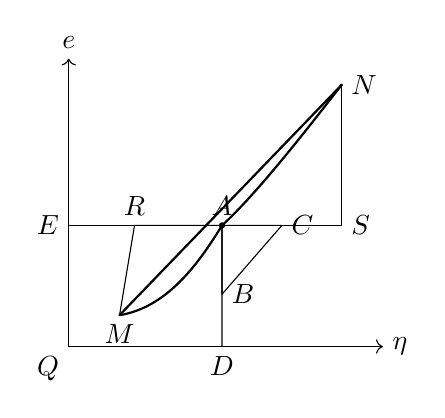
\begin{tikzpicture}[scale=.95, line cap=round, line join=round]
  \coordinate (Q) at (0,0);
  \coordinate (E) at (0,1.62);
  \coordinate (A) at (2.05,1.62);
  \coordinate (D) at (2.05,0);
  \coordinate (B) at (2.05,.70);
  \coordinate (C) at (2.85,1.62);
  \coordinate (S) at (3.65,1.62);
  \coordinate (N) at (3.65,3.50);
  \coordinate (M) at (.68,.42);
  \coordinate (R) at (.88,1.62);
  \draw[->] (Q)--(0,3.85) node[above] {$e$};
  \draw[->] (Q)--(4.20,0) node[right] {$\eta$};
  \draw[thick] (M).. controls (1.30,.52) and (1.72,1.08)..(A).. controls (2.50,2.03) and (3.12,2.82)..(N);
  \draw[thick] (M)--(N);
  \draw (E)--(S)--(N);
  \draw (M)--(R)--(A)--(D);
  \draw (A)--(C)--(B)--(A);
  \fill (A) circle (1.2pt);
  \node[left] at (E) {$E$};
  \node[above] at (R) {$R$};
  \node[above] at (A) {$A$};
  \node[right] at (C) {$C$};
  \node[right] at (S) {$S$};
  \node[right] at (N) {$N$};
  \node[below] at (M) {$M$};
  \node[right] at (B) {$B$};
  \node[below] at (D) {$D$};
  \node[below left] at (Q) {$Q$};
\end{tikzpicture}
\caption{Fig. 3.}
\end{figure}

The relations of these quantities to one another and to the surface of dissipated energy are illustrated by figure 3, which represents a plane perpendicular to the axis of $v$ and passing through the point $A$, which represents the initial state of the body. $MN$ is the section of the surface of dissipated energy. $Qe$ and $Q\eta$ are sections of the planes $\eta=0$ and $e=0$, and therefore parallel to the axes of $e$ and $\eta$ respectively. $AD$ and $AE$ are the energy and entropy of the body in its initial state, $AB$ and $AC$ its available energy and its capacity for entropy respectively. It will be observed that when either the available energy or the capacity for entropy of the body is $0$, the other has the same value. Except in this case, either quantity may be varied without affecting the other. For, on account of the curvature of the surface of dissipated energy, it is evidently possible to change the position of the point representing the initial state of the body so as to vary its distance from the surface measured parallel to one axis without varying that measured parallel to the other.

As the different sense in which the word entropy has been used by different writers is liable to cause misunderstanding, it may not be out of place to add a few words on the terminology of this subject. If Professor Clausius had defined entropy so that its value should be determined by the equation
\[
dS=-\frac{dQ}{T},
\]
instead of his equation (\emph{Mechanische W\"armetheorie}, Abhand. ix. \S 14; \emph{Pogg. Ann.}, July, 1865)
\[
dS=\frac{dQ}{T},
\]
where $S$ denotes the entropy and $T$ the temperature of a body and $dQ$ the element of heat imparted to it, that which is here called capacity for entropy would naturally be called available entropy, a term the more convenient on account of its analogy with the term available energy. Such a difference in the definition of entropy would involve no difference in the form of the thermodynamic surface, nor in any of our geometrical constructions, if only we suppose the direction in which entropy is measured to be reversed. It would only make it necessary to substitute $-\eta$ for $\eta$ in our equations, and to make the corresponding change in the verbal enunciation of propositions. Professor Tait has proposed to use the word entropy ``in the opposite sense to that in which Clausius has employed it'' (\emph{Thermodynamics}, \S 48. See also \S 178), which appears to mean that he would determine its value by the first of the above equations. He nevertheless appears subsequently to use the word to denote available energy (\S 182, 2d theorem). Professor Maxwell uses the word entropy as synonymous with available energy, with the erroneous statement that Clausius uses the word to denote the part of the energy which is not available (\emph{Theory of Heat}, pp. 186 and 188). The term entropy, however, as used by Clausius does not denote a quantity of the same kind (i.e., one which can be measured by the same unit) as energy, as is evident from his equation, cited above, in which $Q$ (heat) denotes a quantity measured by the unit of energy, and as the unit in which $T$ (temperature) is measured is arbitrary, $S$ and $Q$ are evidently measured by different units. It may be added that entropy as defined by Clausius is synonymous with the thermodynamic function as defined by Rankine.

Thirdly. A certain initial condition of the body is given as before. No work is allowed to be done upon or by external bodies, nor any heat to pass to or from them; from which conditions bodies may be excepted, as before, in which no permanent changes are produced. It is required to find the amount by which the volume of the body can be diminished, using for that purpose, according to the conditions, only the force derived from the body itself. The conditions require that the energy of the body shall not be altered nor its entropy diminished. Hence the quantity sought is represented by the distance of the point representing the initial state from the surface of dissipated energy, measured parallel to the axis of volume.

Fourthly. An initial condition of the body is given as before. Its volume is not allowed to be increased. No work is allowed to be done upon or by external bodies, nor any heat to pass to or from them, except a certain body of given constant temperature $t'$. From the latter conditions may be excepted as before bodies in which no permanent changes are produced. It is required to find the greatest amount of heat which can be imparted to the body of constant temperature, and also the greatest amount of heat which can be taken from it, under the supposed conditions. If through the point of the

initial state a straight line be drawn in the plane perpendicular to the axis of $v$, so that the tangent of the angle which it makes with the direction of the axis of $\eta$ shall be equal to the given temperature $t'$, it may easily be shown that the vertical projections of the two segments of this line made by the point of the initial state and the surface of dissipated energy represent the two quantities required.\footnote{Thus, in figure 3, if the straight line $MAN$ be drawn so that $\tan NAC=t'$, $MR$ will be the greatest amount of heat which can be given to the body of constant temperature and $NS$ will be the greatest amount which can be taken from it.}

These problems may be modified so as to make them approach more nearly the economical problems which actually present themselves, if we suppose the body to be surrounded by a medium of constant pressure and temperature, and let the body and the medium together take the place of the body in the preceding problems. The results would be as follows:

If we suppose a plane representing the constant pressure and temperature of the medium to be tangent to the surface of dissipated energy of the body, the distance of the point representing the initial state of the body from this plane measured parallel to the axis of $e$ will represent the available energy of the body and medium, the distance of the point to the plane measured parallel to the axis of $\eta$ will represent the capacity for entropy of the body and medium, the distance of the point to the plane measured parallel to the axis of $v$ will represent the magnitude of the greatest vacuum which can be produced in the body or medium (all the power used being derived from the body and medium); if a line be drawn through the point in a plane perpendicular to the axis of $v$, the vertical projection of the segment of this line made by the point and the tangent plane will represent the greatest amount of heat which can be given to or taken from another body at a constant temperature equal to the tangent of the inclination of the line to the horizon. (It represents the greatest amount which can be given to the body of constant temperature, if this temperature is greater than that of the medium; in the reverse case, it represents the greatest amount which can be withdrawn from that body.) In all these cases, the point of contact between the plane and the surface of dissipated energy represents the final state of the given body.

If a plane representing the pressure and temperature of the medium be drawn through the point representing any given initial state of the body, the part of this plane which falls within the surface of dissipated energy will represent in respect to volume, entropy, and energy all the states into which the body can be brought by reversible processes, without producing permanent changes in external bodies (except in the medium), and the solid figure included between

this plane figure and the surface of dissipated energy will represent all the states into which the body can be brought by any kind of processes, without producing permanent changes in external bodies (except in the medium).\footnote{The body under discussion has been supposed throughout this paper to be homogeneous in substance. But if we imagine any material system whatever, and suppose the position of a point to be determined for every possible state of the system, by making the co-ordinates of the point equal to the total volume, entropy, and energy of the system, the points thus determined will evidently form a solid figure bounded in certain directions by the surface representing the states of dissipated energy. In these states, the temperature is necessarily uniform throughout the system; the pressure may vary (e.g., in the case of a very large mass like a planet), but it will always be possible to maintain the equilibrium of the system (in a state of dissipated energy) by a uniform normal pressure applied to its surface. This pressure and the uniform temperature of the system will be represented by the inclination of the surface of dissipated energy according to the rule on page 34. And in regard to such problems as have been discussed in the last five pages, this surface will possess, relatively to the system which it represents, properties entirely similar to those of the surface of dissipated energy of a homogeneous body.}

\end{document}
